% !TEX root = ../notes.tex
\section{Harvesting a single natural population}
\marginnote{\emph{Lecture 7}}[0mm]
We are now going to move into another example and consider different types of bifurcation. We are going to now consider a harvesting,
$$ \di N t = rN \left( 1 - \frac{N }{k} \right) - h(N) $$
where $h(N)$ is our harvesting rate. Initially we are going to keep it simple and let $h$ be our harvesting rate, $h(N) = hN$. Now look for steady states,
$$ rN \left( 1 - \frac{N }{k}\right) - hN = 0 $$
which has solutions, $N^* = 0$ and $r - \frac{rN^{**w}}{k} - h =0$, hence, $N^{**} = k\left( 1 - \frac{h }{r} \right)$. \\
We can consider $f(N) = F(N) - G(N)$ where $F(N) = rN \left( 1 - \frac{N }{k} \right)$ and $G(N) = hN$ and then plot them.

\begin{figure}[!ht]
\centering
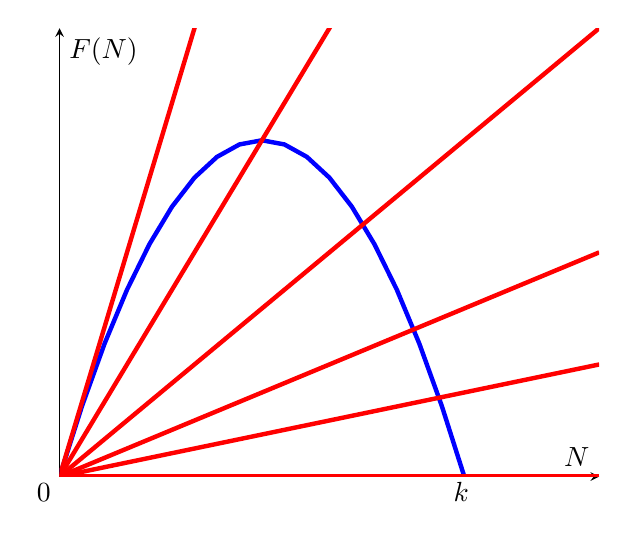
\begin{tikzpicture}[scale=1.0]
\begin{axis}[
        ticks = none,
        axis x line=middle,
        axis y line=middle,
        ymax=1, ymin=0, ylabel=$F(N)$,
        xlabel=$N$
        ]
    \addplot[domain=0:4, blue, ultra thick] {x * (1 - x/3)};
    \addplot[domain=0:4, red, ultra thick] {x};
    \addplot[domain=0:4, red, ultra thick] {x/2};
    \addplot[domain=0:4, red, ultra thick] {x/4};
    \addplot[domain=0:4, red, ultra thick] {x/8};
    \addplot[domain=0:4, red, ultra thick] {x/16};
    \addplot[domain=0:4, red, ultra thick] {0};
\end{axis}
\node at (-0.2, -0.2) {$0$};
\node at (5.1, -0.2) {$k$};w
\end{tikzpicture}
\caption{}
\end{figure}

\noindent
We can find the stability, firstly consider $f'(N) = r - h - \frac{2t }{k}N$ and see $f'(0) = r - h$ and $f'(N^*) = h - r$. We notice that for a positive steady state at $N^{**}$ we need $h < r$. So assume that $h < r$, then we can see that we have $f'(0) > 0$ and $f'(N^{*}) < 0$ and so we call the $h < r$ sustainable harvesting. \\
In actuality, we want some yield. We denote yield, $Y(h) = nN_h$ where $N_h = N^{**}$. Hence we write $y(h)$,
$$ y(h) = hk\left( 1 - \frac{h}{r}\right) $$
this is a quadratic and so we have a control parameter $h$. Given it's a parabola we can find a maximum yield bt finding the maxima of the parabola. This occurs at $h = \frac{r }{2}$ and the yield is, $\frac{rk}{4}$. We can also find the value of $N_h$, which is $N_h = \frac{k}{2}$. These are the two values we expect for the logistic curve. \\

\noindent
We can vary $h$ and when $h = 0$ we can just see that they intersect at $(0, k)$ and it's not that interesting. Then as $h$ increases it heads towards the $\frac{k }{2}$ and this is a critical value, as we see in Figure 9. Now imagine we increase the slope further then we reach the point where they are tangential. Over the varying of $h$ we can see that the stability changes, after the tangential behavior they meet again for negative $N$ and creates a new saddle point.

\newpage
\subsection{Transcritical Bifurcation}
Before, we reached a point where the steady states absorb eachother. Here we have places where they meet and then don't absorb eachother. Here is the diagram;
\begin{figure}[!ht]
\centering
\begin{tikzpicture}[scale=1.0]
\begin{axis}[
        ticks = none,
        axis x line=middle,
        axis y line=middle,
        ymax=1.25, ymin=0,
        xlabel=$h$
        ]
\end{axis}
\draw (0, 0) circle (0.1);
\draw (1, 0) circle (0.1);
\draw (2, 0) circle (0.1);
\draw (3, 0) circle (0.1);
\draw (4, 0) circle (0.1);
\draw (5, 0) circle (0.1);
\fill (6, 0) circle (0.1);
\fill (0, 5) circle (0.1);
\fill (1, 4) circle (0.1);
\fill (2, 3) circle (0.1);
\fill (3, 2) circle (0.1);
\fill (4, 1) circle (0.1);
\draw (6, -1) circle (0.1);
\end{tikzpicture}
\caption{Bifuration Diagram for our system}
\end{figure}

Consider $\di N t = f(N, k)$ where $k$ is a parameter. There is a critical value of $k$, $k_c$ such that when $k = k_c$ then $f'(N^*) = 0$ for some $N^*$.
\begin{ndefi}[Transcritical Bifurcation]
  Then the bifurcation at $k_c$ is transcritical if as $k$ passes through the stable-unstable pair of equilibria collide and exchange stability.
\end{ndefi}

\noindent
Whenever $k < k_c$ we have stable node and an unstable node. We go from harvesting state was supporting the population to depletion at $k = k_c$.

We now consider another factor, the time response. We define this as $T_R = \frac{1}{|f'(N^*)|}$. We say that the sign of the derivative denotes the stability of the point but the inverse maginitude is the time it takes the perturbation to return to normal. If we remove something from the population, will it take ages to get back to normal? Firslt consider the non-zer steady state. We saw that $f'(N_h) = h - r$, and we know that $h < r$ and so, $T_R(h) = \frac{1 }{r - h }$ and when $h = 0$, $T_r (h = 0) = \frac{1 }{r}$.\\

\noindent
\begin{ndefi}[Relative Recovery Time]
  We define simply the relative recovery time as,
  $$ \frac{T_R (h)}{T_R(h = 0)} $$
\end{ndefi}
and s the relative recovery time for our system at $N_h$ is simply,
$$ RRT = \frac{r}{r - h} $$
We can now start to look at the relation between yield and the relative recovery time and yield.

\subsection{RRT and yield}
We remember that $y(t) = hk\left( 1 - \frac{h }{r}\right)$ and we can then write $h^2 - rh + \frac{rY}{k} = 0$. Hence by the quadratic formula, $h = \frac{r }{2} \left( 1 + \sqrt{1 - \frac{4Y}{rK}}\right)$ and now as we know our maximum yield is simply just $\frac{rk }{4}$, then we can say, $h = \frac{r }{2} \left( 1 + \sqrt{1 - \frac{Y}{Y_{max}}}\right)$.
Hence, now we go to recovery time.
$$ T_R(h) = \frac{1}{r - h} = \frac{1}{r - \frac{r }{2} \left( 1 \pm \sqrt{1 - \frac{Y}{Y_{max}}}\right)} $$
and now the relative recovery time.
$$ RRT(Y) = \frac{2}{1 \pm \sqrt{ 1 - \frac{Y}{Y_{max}}}} $$

\marginnote{\emph{Lecture 7}}[0mm]
We split our RRT into two branches, $L_+$ and $L_-$. We also note that $0 \le \frac{Y}{Y_{max}} \le 1$. If $\frac{Y }{Y_{max}} = 1$, then, $L_+ = 1$. Hence, we can plot this RRT function.

\begin{figure}[!ht]
\centering
\begin{tikzpicture}[scale=1.0]
\begin{axis}[
        ticks = none,
        axis x line=middle,
        axis y line=middle,
        ymax=1.25, ymin=0,
        xlabel=$\frac{Y}{Y_{max}}$
        ]
\end{axis}
\draw [thick] plot [smooth, tension = 1] coordinates { (0, 1) (4, 1.3) (5, 2)};
\draw [thick, red] plot [smooth, tension = 1] coordinates { (5, 2) (2, 3) (0.3, 5.6)};
\node at (5, -0.3) {1};
\node at (-0.1, -0.3) {0};
\node at (-0.3, 2) {2};
\node at (-0.3, 1) {1};
\node at (4, 1.6)  {$L_+$};
\node at (2, 2.7) {\color{red} $L_-$};
\end{tikzpicture}
\caption{RRT for different values of $\frac{Y}{Y_{max}}$}
\end{figure}
This relates to as you go further and further towards the $(0, 0)$ steady state you go off to infinity.

\newpage
\subsection{Constant Yield Harvesting}
We use the same model as before, but now we let $f(N) = N_0$. Then we can find the steady states and we get a quadratic which we can them solve and get our steady states $N = \frac{1}{2}\left(k \pm \sqrt{k^2 - \frac{4kY_0}{r}}\right) = \frac{k }{2}\left( 1 \pm \sqrt{1 - \frac{4Y_0}{kr}} \right)$ and now again we consider $f(N) = g(N) - Y_0$.

\begin{figure}[!ht]
\centering
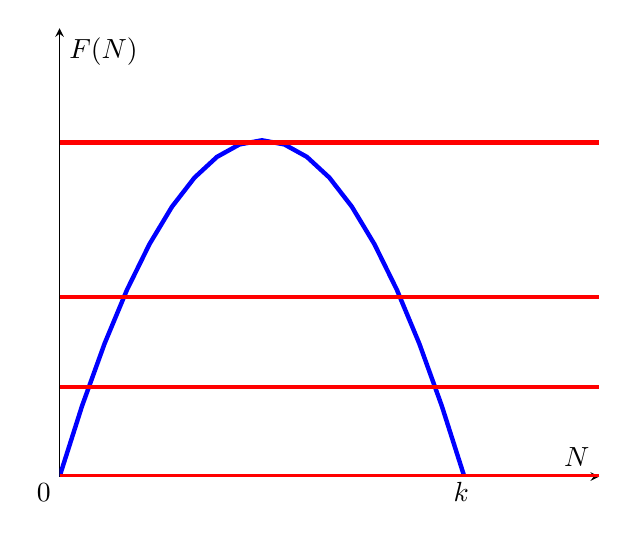
\begin{tikzpicture}[scale=1.0]
\begin{axis}[
        ticks = none,
        axis x line=middle,
        axis y line=middle,
        ymax=1, ymin=0, ylabel=$F(N)$,
        xlabel=$N$
        ]
    \addplot[domain=0:4, blue, ultra thick] {x * (1 - x/3)};
    \addplot[domain=0:4, red, ultra thick] {0};
    \addplot[domain=0:4, red, ultra thick] {0.2};
    \addplot[domain=0:4, red, ultra thick] {0.4};
    \addplot[domain=0:4, red, ultra thick] {0.745};
\end{axis}
\node at (-0.2, -0.2) {$0$};
\node at (5.1, -0.2) {$k$};w
\end{tikzpicture}
\caption{}
\end{figure}

When $Y_0 = 0$, we get two steady states, one saddle point at $0$ and a stable node at $N^*$. When we have a tangent line, then $f'(N) = 0$ at that point and we have a bifurcation there. We notice here, again, we have a saddle node bifurcation.\\

\noindent
Now we consider the time response, we can see that $f'(N) = r - \frac{2rN}{k}$ and so,
\begin{align*}
  T_R(N_+) &= \frac{1}{r\sqrt{1 - \frac{Y_0}{Y_{max}}}}\\
  RRT = \frac{1}{\sqrt{1 - \frac{Y_0}{Y_{max}}}}
\end{align*}
and then we get an asymptote and so RRT goes to infinity. However there are several problems to what we are going here, as we head towards the tangential line, there may be a point where it jumps from one point to another. At other points, it can't jump as it's further apart.

\section{Interactive Populations}
We are now going to jump to 2D,
\begin{eg}
  Let's model the density of  $N(t)$ which is our population of prey and $P(t)$ be the population of predators.
  \begin{align*}
    \di N t &= rN\left( 1 - \frac{N }{k} \right) - NPR(N)\\
    \di P t &= sN \left( 1 - \frac{P }{hN} \right)
  \end{align*}
  We know need to choose $R(N)$, so we want a curve where we start at $(0, 0)$ and asymptotes for large $N$. We let it be a $R(N) = \frac{k }{N + D}$, hence our system is:
  \begin{align*}
    \di N t &= rN\left( 1 - \frac{N }{k} \right) - \frac{kNP}{N + D}\\
    \di P t &= sN \left( 1 - \frac{P }{hN} \right)
  \end{align*}
  We can now consider the steady states of $di N t$ and so we can seek to non-dimensionalise it. 
\end{eg}
